\chapter{Capitolo 4: Algoritmi basati sulla distanza}
In questo capitolo vengono illustrati i principali algoritmi utilizzati per la costruzione degli alberi evolutivi. L'obiettivo è quello di trovare una soluzione al cosiddetto \textit{problema degli alberi basati sulla distanza}, ma prima è necessario introdurre alcuni concetti, tra cui la matrice delle distanze.

\section{Matrice delle distanze}
Dati due punti, $x$ e $y$, la \textit{distanza} può essere vista come loro "lontananza" in uno spazio $k$-dimensionale. Nella fattispecie, è una funzione $d(x,y)$ che possiede le seguenti proprietà \cite{molaCagliari}:
\begin{enumerate}
	\item \textit{non negatività}:
	\[d(x,y)\geq 0\hspace{2em} \forall \: x,y\in R^k\]
	\item \textit{identità}:
	\[d(x,y)=0 \; \leftrightarrow \; x=y\]
	\item \textit{simmetria}:
	\[d(x,y)=d(y,x)\hspace{2em} \forall \: x,y\in R^k\]
	\item \textit{disuguaglianza triangolare}:
	\[d(x,y)\leq d(x,z)+d(y,z)\hspace{2em} \forall \: x,y,z\in R^k\]
\end{enumerate}
Date $n$ unità, calcolando la distanza per ogni coppia di elementi\footnote{Ci sono vari modi per calcolare la distanza tra una coppia di elementi, ad esempio attraverso la distanza Euclidea, quella di Manhattan, di Minkowski e così via.} si ottiene una \textit{matrice delle distanze $n \times n$}, definita nel seguente modo \cite{ingrassiaStatistica}:
\[
D = \begin{pmatrix}
0 & d_{12} & d_{13} & \ldots & d_{1n} \\ 
d_{21} & 0 & d_{23} & \ldots & d_{2n} \\ 
d_{31} & d_{32} & 0 & \ldots & d_{3n} \\ 
\vdots & \vdots & \vdots & \ddots & \vdots \\ 
d_{n1} & d_{n2} & \ldots & \ldots & 0
\end{pmatrix}
\hspace{3em}dove\;d(x_i,x_j)=D_i,_j
\]
Poiché è costruita a partire dalle distanze, ne eredita le proprietà precedentemente elencate.
\newline
Ciascun valore $D_i,_j$ può assumere significati diversi in base al contesto, ad esempio, può indicare il numero di simboli diversi tra i geni $i$ e $j$ nell'allineamento di sequenze di DNA\footnote{'allineamento è il processo attraverso il quale si misura la similarità tra due o più sequenze.}, come mostrato nell'esempio sottostante:
\begin{figure}[h!]
	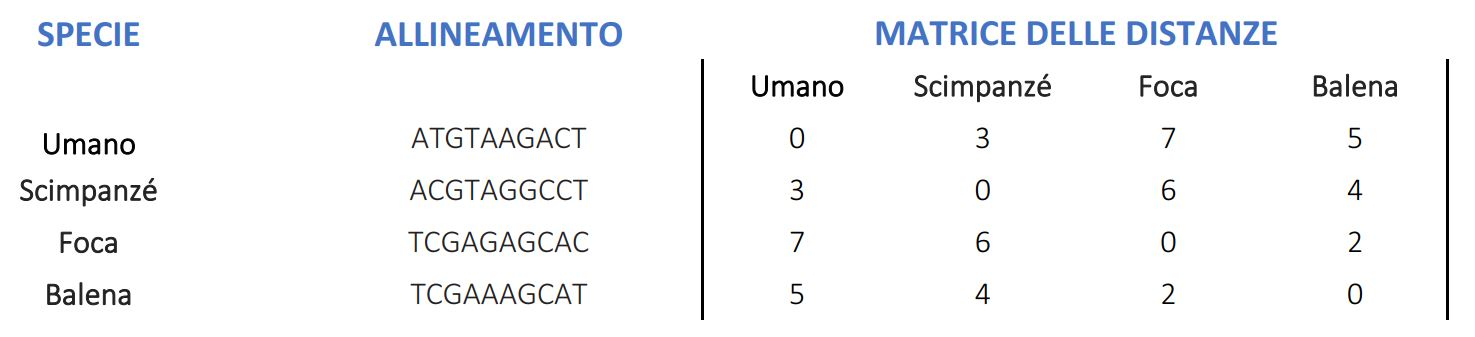
\includegraphics[width=\linewidth]{distance_matrix_example.jpg}
 	\caption{Esempio di matrice delle distanze.}
  	\label{fig:DistanceMatrix}
\end{figure}
\newline
Dalla figura 5 è possibile notare che la sequenza di DNA della foca risulta molto più simile a quella della balena, in quanto la distanza è $2$, piuttosto che con l'umano, la cui distanza invece è $7$.
\newpage

\section{Problema degli alberi basati sulla distanza}
Gli algoritmi basati sulla distanza utilizzano la matrice delle distanze per costruire gli alberi evolutivi, dove le foglie corrispondono alle entità biologiche presenti nella matrice, mentre i nodi interni rappresentano gli antenati non noti. Per poter conoscere quale è la distanza tra due foglie, e quindi conoscere quanto sono legate tra loro, è necessario associare un valore non negativo (peso) a ciascun arco, pertanto la lunghezza del cammino in tale albero è la somma dei suoi pesi. Si definisce, quindi, la \textit{distanza evolutiva} tra due entità biologiche corrispondenti alle foglie $i$ e $j$ di un albero $T$ come la lunghezza dell'unico cammino che li collega, ed è indicato come $d_i,_j(T)$ \cite{bioinfalganactivelearningapproachparttwo}. In altre parole è dato dalla somma dei pesi degli archi che ci sono tra $i$ e $j$.
\newline
Si dice che un albero $T$ si \textit{adatta} ad una matrice delle distanze $D$ se per ogni coppia di foglie $i$ e $j$ si ha che $D_i,_j=d_i,_j(T)$, ovvero l'elemento nella riga $i$ e colonna $j$ è uguale alla lunghezza del cammino che le collega (distanza evolutiva), in tal caso la matrice viene definita \textit{additiva}. Qualora invece non esista un albero che si adatti alla matrice, allora è \textit{non additiva}.
\newline
Si riporta di seguito un esempio che mostra un albero che si adatta alla matrice delle distanze mostrata nella sezione precedente.
\begin{figure}[h!]
	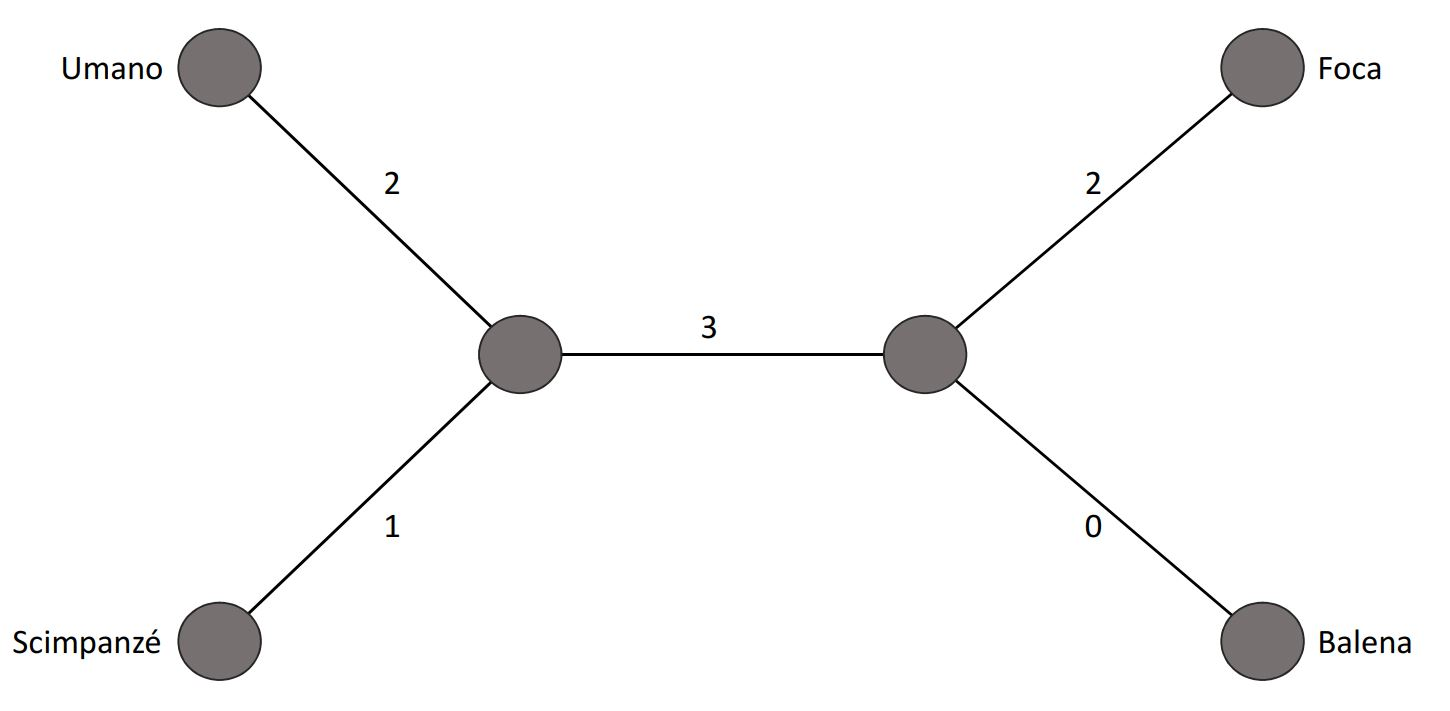
\includegraphics[width=\linewidth]{unrooted_tree_created_by_figure_5.jpg}
 	\caption{Albero evolutivo senza radice costruito a partire dalla matrice \textbf{adattiva} della figura 5.}
  	\label{fig:EvolutionaryTreeExample}
\end{figure}
\newline
Ci possono essere più alberi che si adattano ad una matrice, quindi come si può scegliere l'albero giusto? Si nota che quello in figura 6 ha tutti i vertici di grado diverso da due e viene definito \textit{albero semplice}. 
\newpage
Una loro caratteristica importante è che per ogni matrice delle distanze adattiva esiste un unico albero semplice che si adatta alla matrice stessa.
\newline
Adesso è possibile dare una definizione al problema accennato all'inizio del capitolo:
\begin{center}
\textbf{Problema degli alberi basati sulla distanza:}
\newline
\textit{Dato in \textbf{input} una matrice delle distanze adattiva si ottiene in \textbf{output} un albero evolutivo semplice.}
\end{center}

\section{Algoritmo per il problema degli alberi basati sulla distanza}
L'obiettivo è quello di costruire un albero semplice $T$ che si adatti alla matrice delle distanze $D$.
\newline
Si prenda in considerazione la matrice delle distanze mostrata nella figura 5 e riportata di seguito\footnote{Per brevità si definisce ,u=umano, s=scimpanzé, f=foca, b=balena.}:
\[
D = \bordermatrix{\text{specie}&u&s&f&b\cr
                u& 0 & 3 & 7 & 5\cr
                s& 3 & 0 & 6 & 4\cr
                f& 7 & 6 & 0 & 2\cr
                b& 5 & 4 & 2 & 0}
\]
\newline
L'idea di base dell'algoritmo è che le specie che sono più vicine tra loro nella matrice siano effettivamente i \textit{vicini} nel rispettivo albero e quindi abbiano lo stesso genitore, con $D_i,_j=d_i,_j(T)$.
\newline
Poiché l'elemento più piccolo della matrice è $D_{fb}$, la cui distanza evolutiva è $2$, possiamo supporre che $f$ e $b$ siano vicini. Si indica con $p$ il genitore non noto delle due foglie. La situazione è mostrata di seguito.
\begin{figure}[h!]
\centering
	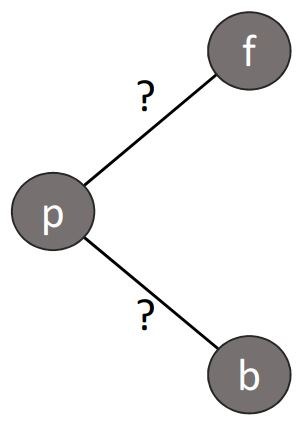
\includegraphics[height=3cm, width=2cm]{distance_between_f_b.jpg}
 	\caption{Foglie vicine con un generico genitore $p$.}
  	\label{fig:neighborsleaves}
\end{figure}
\newline
Come si può calcolare la distanza tra $f$, $p$ ($d_{fp}$) e tra $b$, $p$ ($d_{bp}$) ? Le uniche informazioni a disposizione sono le distanze tra le quattro foglie presenti nella matrice e che $f$, $p$ sono vicini. Il passo successivo dell'algoritmo è mostrato di seguito.
\begin{figure}[h!]
\centering
	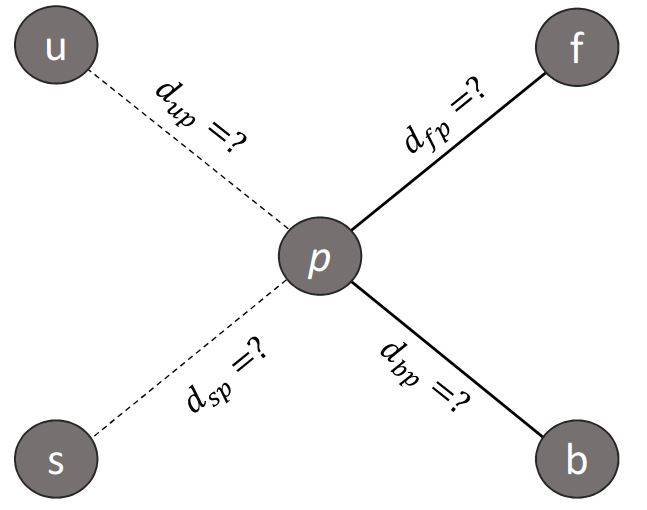
\includegraphics[height=9cm, width=7cm, keepaspectratio]{distance_between_f_b_part_2.jpg}
 	\caption{Le quattro foglie $u$, $s$, $f$ e $d$.}
  	\label{fig:neighborsleaves_2}
\end{figure}
\newline
Nella figura 8 sono state aggiunte le foglie $u$ ed $s$, ma il loro arco è tratteggiato in quanto ancora non è possibile sapere come sono collocate nell'albero.
\newline
Viene scelta una casualmente una foglia tra $u$ ed $s$ e viene sfruttato il valore della sua distanza rispetto alle altre foglie per poter calcolare $d_{fp}$ e $d_{bp}$ (in questo caso si sceglie $u$). Per far ciò è quindi necessario scrivere le distanze tra le foglie nel seguente modo:
\[d_{fu}=d_{fp}+d_{up}\]
\[d_{fb}=d_{fp}+d_{bp}\]
\[d_{bu}=d_{bp}+d_{up}\]
\[d_{up}=\frac{d_{fu}+d_{bu}-d_{fb}}2=
\frac{(d_{fp}+d_{up})+(d_{bp}+d_{up})-(d_{fp}+d_{bp})}2=\]
\[=\frac{d_{fp}+d_{up}+d_{bp}+d_{up}-d_{fp}-d_{bp}}2=
\frac{d_{up}+d_{up}}2=
\frac{2d_{up}}2=d_{up}
\]
Perché scrivere $d_{up}$ in quel modo? perché non si conosce il peso dei nodi interni, ma solo quello delle foglie, grazie alla matrice di partenza. Ma allora $d_{fu}=D_{fu}$, $d_{fb}=D_{fb}$, $d_{bu}=D_{bu}$, quindi si può scrivere $d_{up}$ nel seguente modo:
\[d_{up}=\frac{d_{fu}+d_{bu}-d_{fb}}2=\frac{D_{fu}+D_{bu}-D_{fb}}2\]
A questo punto si è in grado di calcolare la distanza tra $f$ e $p$ e tra $b$ e $p$, ricavandoli dalle uguaglianze di cui sopra. Per prima cosa si trova $d_{fp}$:
\[d_{fu}=d_{fp}+d_{up} \rightarrow d_{fp}=d_{fu}-d_{up}=D_{fu}-D_{up}=
D_{fu}-\frac{D_{fu}+D_{bu}-D_{fb}}2=\]
\[=\frac{2D_{fu}-D_{fu}-D_{bu}+D_{fb}}2=\frac{D_{fu}+D_{fb}-D_{bu}}2=
\frac{7+2-5}2=2\]
Quindi $d_{fp}=2$. In modo analogo si calcola $d_{bp}$:
\[d_{bu}=d_{bp}+d_{up} \rightarrow d_{bp}=d_{bu}-d_{up}=D_{bu}-D_{up}=
D_{bu}-\frac{D_{fu}+D_{bu}-D_{fb}}2=\]
\[=\frac{2D_{bu}-D_{fu}-D_{bu}+D_{fb}}2=\frac{D_{bu}+D_{fb}-D_{fu}}2=
\frac{5+2-7}2=0\]
Quindi $d_{bp}=0$. Il risultato di questo passo dell'algoritmo è il seguente albero:
\begin{figure}[h!]
\centering
	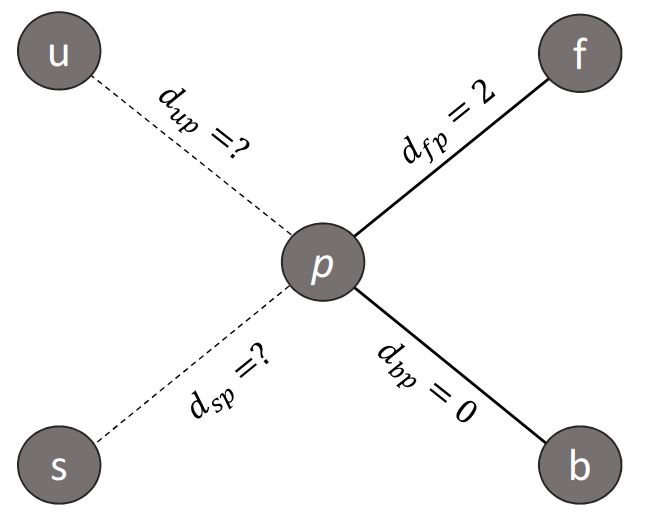
\includegraphics[height=9cm, width=7cm, keepaspectratio]{distance_between_f_b_part_3.jpg}
 	\caption{Albero con le distanze $d_{fp}$ e $d_{bp}$.}
  	\label{fig:neighborsleaves_3}
\end{figure}
\newline
Il prossimo step consiste nel trovare la distanza tra $u$ e $p$ e tra $s$ e $p$. Questo in realtà è semplice: dalla matrice D sappiamo che $D_{fu}=d_{fu}=7$ e che dai calcoli precedenti che $d_{fp}=2$, quindi $d_{up}=d_{fu}-d_{fp}=7-2=5$. Stesso ragionamento anche per $d_{sp}$, ovvero $d_{sp}=d_{bs}-d_{bp}=4-0=4$.
\newline
L'albero corrispondente è:
\newpage
\begin{figure}[h!]
\centering
	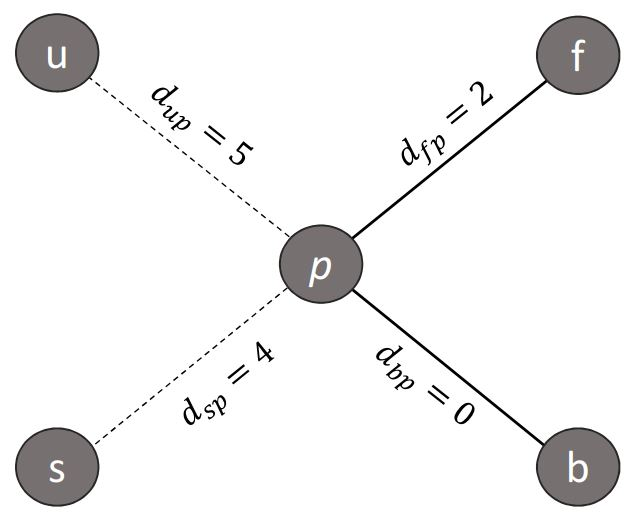
\includegraphics[height=9cm, width=7cm, keepaspectratio]{distance_between_f_b_part_4.jpg}
 	\caption{Albero con le distanze $d_{fp}$, $d_{bp}$, $d_{up}$ e $d_{sp}$.}
  	\label{fig:neighborsleaves_3}
\end{figure}
Adesso è necessario fare due modifiche alla matrice D, la prima consiste nel mettere una riga e colonna in più, definite $p$, che rappresentano i valori appena calcolati, ottenendo quindi la seguente matrice:
\[
D = \bordermatrix{\text{specie}&u&s&f&b&p\cr
                u& 0 & 3 & 7 & 5 & 5\cr
                s& 3 & 0 & 6 & 4 & 4\cr
                f& 7 & 6 & 0 & 2 & 2\cr
                b& 5 & 4 & 2 & 0 & 0\cr
                p&  5 & 4 & 2 & 0 & 0}
\]
la seconda invece consiste nel togliere le righe e colonne appartenenti a $f$ e $b$, in quanto già aggiunti all'albero e quindi non più utili. Quindi:
\[
D = \bordermatrix{\text{specie}&u&s&p\cr
                u& 0 & 3 & 5\cr
                s& 3 & 0 & 4\cr
                p&  5 & 4 & 0}
\]
Anche se adesso si conoscono le distanze di tutte le foglie con il genitore $p$, rimane comunque da capire se le altre due foglie, ovvero $u$ e $s$ abbiano altri genitori. Si ricorda, infatti che i loro archi sono stati tratteggiati in quanto ancora non si conosce la loro collocazione nell'albero.
Per risolvere questo problema basta applicare ricorsivamente i passi precedenti, quindi si individua l'elemento più piccolo della matrice ($d_{su}$) e si suppone che essi siano vicini e quindi che abbiano un genitore non noto $k$, come mostrato in figura 11.
\newpage
\begin{figure}[h!]
\centering
	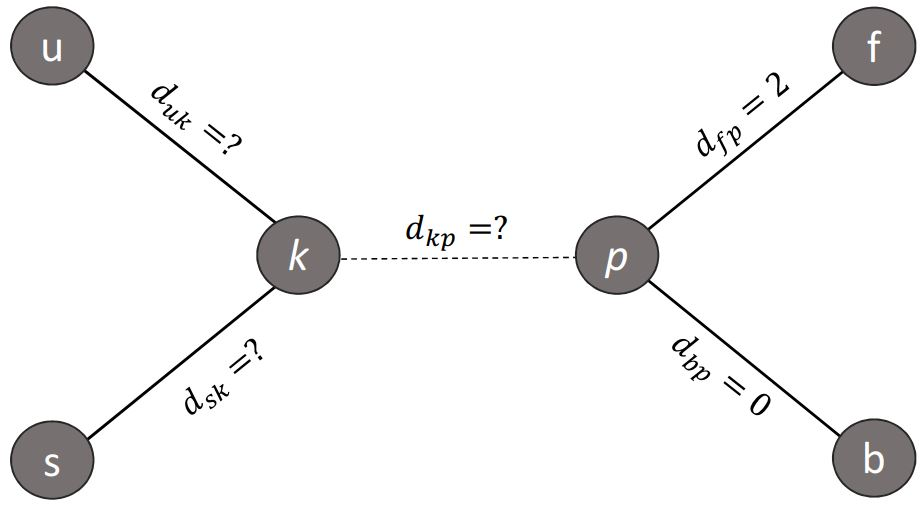
\includegraphics[height=13cm, width=11cm, keepaspectratio]{distance_between_s_u.jpg}
 	\caption{Albero con le nuove distanze da calcolare.}
  	\label{fig:neighborsleaves_3}
\end{figure}
Viene scelto il nodo $p$ e sfruttato il valore della sua distanza rispetto alle altre foglie per poter calcolare $d_{uk}$ e $d_{sk}$. Adattando le formule calcolate a pagina $31$ con i dati attuali, si ottiene:
\[d_{pk}=\frac{d_{up}+d_{sp}-d_{us}}2=
\frac{(d_{uk}+d_{pk})+(d_{sk}+d_{pk})-(d_{uk}+d_{sk})}2=\]
\[=\frac{2d_{pk}}2=d_{pk}
\]
Quindi si calcola $d_{uk}$:
\[d_{up}=d_{uk}+d_{pk} \rightarrow d_{uk}=D_{up}-D_{pk}=D_{up}-\frac{D_{up}+D_{sp}-D_{us}}2=\]
\[=\frac{D_{up}+D_{us}-D_{sp}}2=2\]

%-\frac{(D_{uk}+D_{pk})+(D_{sk}+D_{pk})-(D_{uk}+D_{sk})}2=\]
%\[=\frac{(D_{up}+D_{us}-D_{sp})}2=2
%\]
Stessa cosa per $d_{sk}$:
\[d_{sp}=d_{sk}+d_{pk} \rightarrow d_{sk}=D_{sp}-D_{pk}=D_{sp}-\frac{D_{up}+D_{sp}-D_{us}}2=\]
\[=\frac{D_{sp}+D_{us}-D_{up}}2=1\]
Applicando le distanze trovate all'albero della figura 11, si ottiene:
\newpage
\begin{figure}[h!]
\centering
	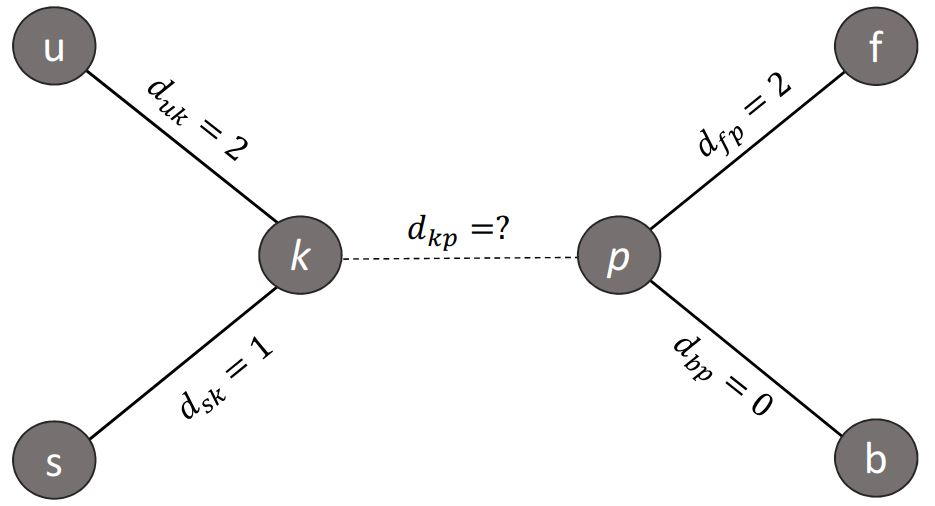
\includegraphics[height=13cm, width=11cm, keepaspectratio]{distance_between_s_u_part_2.jpg}
 	\caption{Albero con le distanze $d_{uk}$ e $d_{sk}$ calcolate.}
  	\label{fig:neighborsleaves_3}
\end{figure}
Dopo aver trovato ricorsivamente la distanza delle foglie dai propri genitori e di conseguenza aver aggiornato la matrice, rimane un ultimo passo da completare, ovvero calcolare la distanza tra $k$ e $p$: in precedenza abbiamo calcolato la distanza tra $u$ e $p$ e tra $s$ e $p$, quindi basta sottrarre tali valori a quelli trovati adesso e troviamo $d_{kp}$.
\[d_{kp}=d_{sp}-d_{sk}=4-1=d_{up}-d_{uk}=5-2=3\]
L'albero finale che si ottiene è il seguente:
\begin{figure}[h!]
\centering
	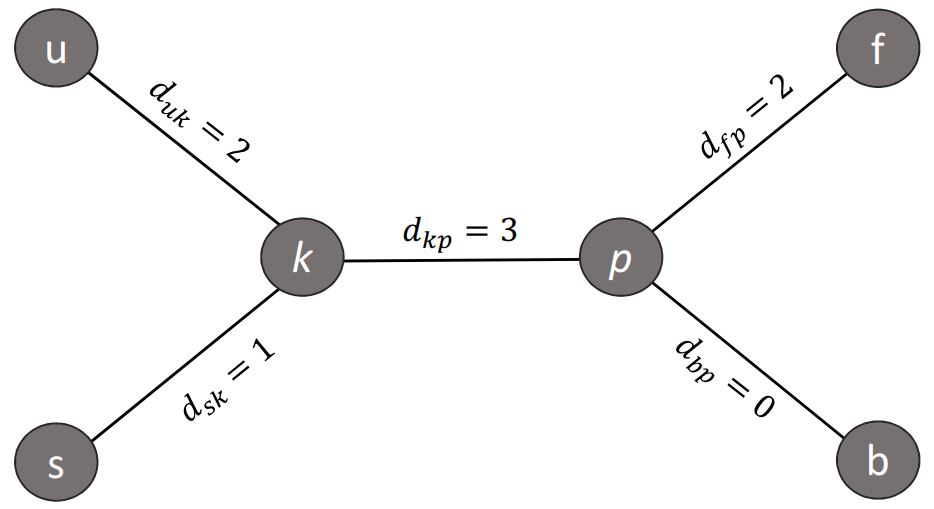
\includegraphics[height=13cm, width=11cm, keepaspectratio]{distance_between_s_u_part_4.jpg}
 	\caption{Albero finale con tutte le distanze calcolate.}
  	\label{fig:neighborsleaves_4}
\end{figure}